% Section content template for individual Educative lessons
% This file contains the actual content for a specific section
% Generated from Educative API section content

% Section: Getting Ready: The Car Rental System
% Section ID: 5816226192556032
% Section Slug: getting-ready-the-car-rental-system
% Generated: 2025-12-12T14:50:09.690850

A \textbf{car rental system} enables customers to rent vehicles for short periods, ranging from a few hours to several weeks. Such systems are commonly operated by companies with multiple offices across cities, often near airports or commercial centers. The platform allows customers to reserve, pick up, and return vehicles at different locations, depending on availability and convenience.
\\
Each branch manages its fleet, consisting of various vehicle types and models, and tracks reservations, customer information, payments, and the logistical aspects of vehicle movement between locations. Customers can search for available vehicles by location, type, or features and reserve or cancel rentals subject to company policies. The system supports multiple payment methods and handles cases such as late returns, reservation modifications, and optional services (e.g., driver assignment and roadside assistance).
\\
This scenario presents several design challenges, including distributed inventory management, concurrent reservations, flexible pickup and drop-off options, dynamic pricing, and ensuring a seamless and reliable customer experience across all locations.
\\
In this LLD interview case study, you'll focus on:

\begin{itemize}
\item
\protect\phantomsection\label{duyeUb8WPc8YPlaGxJaN-}
Managing vehicle inventory and supporting multiple vehicle types and features.
\item
\protect\phantomsection\label{nCGNDuXPUg1e7HbDN3kMo}
Handling reservations, cancellations, and modifications across branches.
\item
\protect\phantomsection\label{7x7I7CEj7UrA0RDvLtELh}
Facilitating vehicle search, pickup, and drop-off at different locations.
\item
\protect\phantomsection\label{Vd0l3X2t4V_rNEvvvszAq}
Tracking customer information, rental history, and payments.
\item
\protect\phantomsection\label{uT1QDvsrRd_AxICpB-7My}
Supporting optional services and flexible payment methods.
\item
\protect\phantomsection\label{NoptirQn0XvcyPtLgftKH}
Ensuring system reliability, data consistency, and scalability.
\end{itemize}
\\
This system model can be adapted for any rental business managing distributed assets and flexible reservations.

\begin{figure}[htbp]
 \centering
 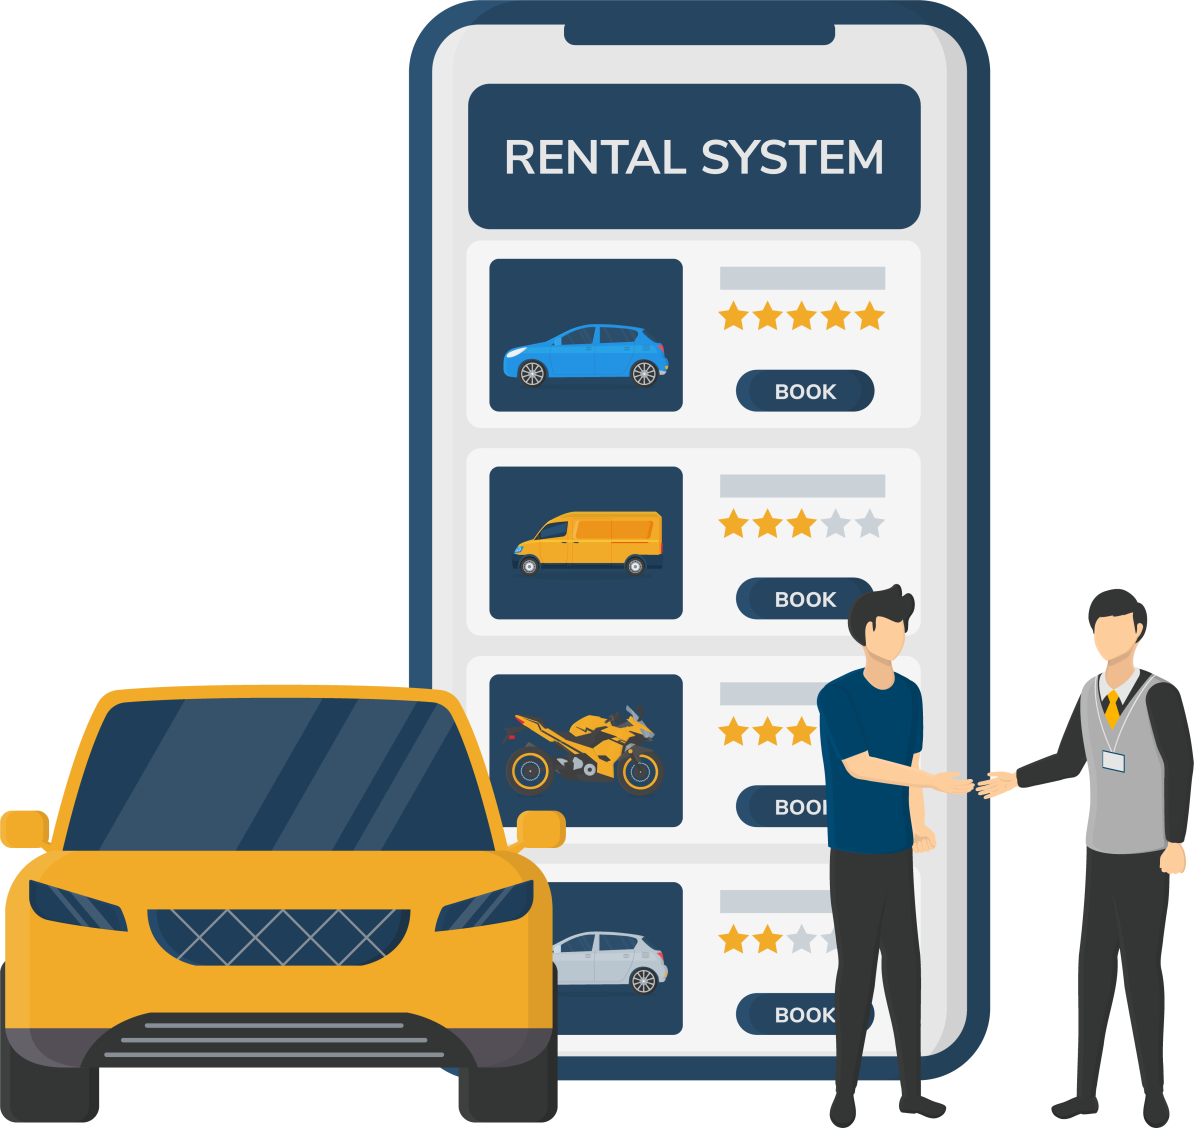
\includegraphics[width=0.15\textwidth]{Images/chapter_15/section_5816226192556032/4710701626294272.png}
 \caption{Application of the car rental system}
\end{figure}

\subsection{Expectations from the interviewee}\label{P0j44cU-Lg3ECyDJANiQ1-2}
\\
The car rental system consists of multiple components with functionality and constraints. This section provides an overview of some of the main expectations that the interviewer will want to hear you discuss in more detail during the interview.

\subsubsection{Vehicle types}\label{Bh90Y7pf1JmAVKnLSNQoa}
\\
An interviewer would expect you to discuss the different vehicle types and ask the following questions:

\begin{itemize}
\item
\protect\phantomsection\label{RQZ0IcHInizNn-xTbbK2j}
What types of vehicles will that system support?
\item
\protect\phantomsection\label{OIzawTREwNhm9z1IVP-G7}
How can we identify the specific vehicle?
\end{itemize}

\subsubsection{Search interface}\label{hLf0joyV01WKZSMj3vGz7}
\\
Members will use the application and add the location and the reservation date. They will receive several options to select the vehicle. Therefore, an interviewer would expect you to ask the questions listed below:

\begin{itemize}
\item
\protect\phantomsection\label{rHczPbnMLvPAE0KY_18PA}
Is it possible to search for a vehicle using its name or type?
\item
\protect\phantomsection\label{12lbpgtKpvM8eBx-at5xz}
Can we search for a vehicle by its model number?
\end{itemize}

\subsubsection{Services}\label{vZZ6b0f9U5IzbdlTUJtoz}
\\
An interviewer would also expect you to discuss the services of the car rental system and may ask the following questions:

\begin{itemize}
\item
\protect\phantomsection\label{-J3KppTQ8-XFf2UggFFc0}
Does a car rental system assign a driver to its customer?
\item
\protect\phantomsection\label{hgusdyRhMxX9OZ52n3M6Y}
Does a car rental system provide roadside assistance to its customers?
\end{itemize}

\subsubsection{Reservation cancellation}\label{An49O3VC7RF8aGSnOL8Zx}
\\
There will be many duplicate instances in our system. The interviewer expects you to ask the questions listed below:

\begin{itemize}
\item
\protect\phantomsection\label{6Z7Ecuz40rta-mQIMgC1k}
Can the member be able to cancel a reservation?
\item
\protect\phantomsection\label{bG0XQtNrByzNaySsTa887}
Which member is allowed to request a vehicle reservation cancellation and when?
\end{itemize}

\subsubsection{Payment flexibility}\label{SZ6vp8e2JoWoYvOGtiz3-}
\\
One of the car rental system's most significant attributes is its customer payment structure. The payment depends on the vehicle type and the time stamp. Therefore, an interviewer would expect you to ask the questions listed below:

\begin{itemize}
\item
\protect\phantomsection\label{6zmiYKcDmeqG1RTk-1gx6}
How can customers pay at different branch locations and by different methods (cash, credit, or cheque)?
\item
\protect\phantomsection\label{5aOsIRrjN9gBx70X-VJLo}
If there are multiple branches of the car rental system, how will the system keep track of customers who have already paid at a particular branch?
\end{itemize}

\subsection{Design approach}\label{DvplzTYkwtkDcfrTaxgUV}
\\
We'll design this car rental system using the bottom-up design approach. For this purpose, we will follow the steps below:

\begin{enumerate}
\item
\protect\phantomsection\label{QH-9Ze9uEP4uNUfZJ9U8d}
\textbf{Identify core components:} Start with basic entities like \texttt{Vehicle}, \texttt{Customer}, \texttt{Reservation}, \texttt{Payment}, etc.
\item
\protect\phantomsection\label{xpy41Wd6tYoh18luCXbkE}
\textbf{Compose subsystems:} Build larger modules for inventory management, reservation management, and payment processing.
\item
\protect\phantomsection\label{BrFbUOqrA6H-PPAsk3_ia}
\textbf{Integrate subsystems:} Assemble the complete application, ensuring the design is modular and adheres to SOLID principles.
\item
\protect\phantomsection\label{VlV3uPQd7XN3o9VXx9x2A}
\textbf{Document assumptions:} Clearly state and justify your assumptions where requirements are unclear.
\end{enumerate}
\\
This design approach will address concurrency and edge cases and follow SOLID principles to ensure scalability and maintainability. Later , diagrams and code will illustrate major workflows and class structures.

\subsection{Design pattern~}\label{vNK0ZMHjkb8rwm-LVZXIE}
\\
During an interview, discussing the design patterns the car rental system falls under is always a good practice. Stating the design patterns gives the interviewer a positive impression and shows that the interviewee is well-versed in the advanced concepts of object-oriented design.
\\
Try to answer the following question. If you are not familiar with design patterns, don't worry! You can learn about them by asking, ``Define design patterns.''

\textbf{Question:}

Which design pattern(s) should be used to design a car rental system? Please elaborate on your choice(s).

Let's explore the requirements of the car rental system in the next lesson.

% End of section content